\documentclass[main.tex]{subfiles}
\newcommand{\DiagramaEscala}{0.9}

\begin{document}

\section{Mathematical Modeling, Numerical Methods, and Problem Solving }

%--------------------------------------------------
% Diapositiva 1
%--------------------------------------------------
\subsection{Modeling, Computers, and Error Analysis}
\begin{frame}{Motivation}
\begin{block}{Por qué recurrir a los métodos numéricos?}
\vspace{0.2cm}
Los métodos numéricos transforman problemas matemáticos en operaciones aritméticas que pueden resolverse con computadoras.\par

\textbf{Clave}: requieren numerosos cálculos tediosos; la disponibilidad de computadoras digitales rápidas ha disparado su uso en ingeniería.
\end{block}

\begin{block}{Impacto del cómputo moderno}
\begin{itemize}
  \item El desarrollo de hardware y software ha incrementado la \emph{potencia de cálculo} accesible.
  \item Permite abordar sistemas \textbf{no lineales}, geometrías complejas y modelos multidimensionales.
  \item Desplaza el esfuerzo desde la ejecución repetitiva de operaciones hacia la \textbf{interpretación creativa} de los resultados.
\end{itemize}
\end{block}
\end{frame}


%--------------------------------------------------
% Diapositiva 2
%--------------------------------------------------
\begin{frame}[c]{Métodos no computacionales}
%\footnotesize
\begin{enumerate}
  \item \textbf{Soluciones analíticas exactas}: útiles para modelos lineales y geometrías simples; limitadas ante la complejidad real.
  \item \textbf{Soluciones gráficas}: empleo de gráficas/monogramas; baja precisión, tediosas sin computadora y restringidas a ≤3~dimensiones.
  \item \textbf{Cálculos manuales de métodos numéricos}: con calculadoras o reglas de cálculo; lentos, propensos a errores y consumen gran esfuerzo.
\end{enumerate}

\begin{block}{Evolución con la llegada de la computadora}
\medskip
Antes, la energía se invertía en la \emph{técnica de cálculo}. Con las computadoras, los métodos numéricos proporcionan soluciones eficientes sin simplificaciones drásticas, liberando tiempo para formular y analizar problemas.
\end{block}
\end{frame}
%--------------------------------------------------
% Diapositiva 3
%--------------------------------------------------
\begin{frame}{Proceso de solución: (a) Antes y (b) Después del uso de computadoras}
\centering
\small
\begin{tikzpicture}[
  box/.style={
    rectangle,
    draw,
    fill=gray!15,
    align=center,
    minimum width=3.6cm,
    minimum height=1.2cm,
    inner sep=2pt
  },
  node distance=1cm,
  >=latex
]

% ---------------- Columna (a) ----------------
\node[box] (a1) {%
  \textbf{FORMULACIÓN}\\
  Leyes fundamentales\\
  explicadas brevemente};

\node[box, below=of a1] (a2) {%
  \textbf{SOLUCIÓN}\\
  Métodos elaborados y a menudo\\
  complicados para manejar el problema};

\node[box, below=of a2] (a3) {%
  \textbf{INTERPRETACIÓN}\\
  Análisis profundo limitado por\\
  una solución que consume tiempo};

\draw[->] (a1) -- (a2);
\draw[->] (a2) -- (a3);

\node at (a3.south) [below=0.1cm] {(a)};

% ---------------- Columna (b) ----------------
\node[box, right=3.5cm of a1] (b1) {%
  \textbf{FORMULACIÓN}\\
  Exposición profunda de la relación\\
  con las leyes fundamentales};

\node[box, below=of b1] (b2) {%
  \textbf{SOLUCIÓN}\\
  Método computacional fácil de usar};

\node[box, below=of b2] (b3) {%
  \textbf{INTERPRETACIÓN}\\
  La capacidad de calcular permite pensar\\
  holísticamente, desarrollar intuición y\\
  estudiar sensibilidad y comportamiento};

\draw[->] (b1) -- (b2);
\draw[->] (b2) -- (b3);

\node at (b3.south) [below=0.1cm] {(b)};

\end{tikzpicture}
\end{frame}


%--------------------------------------------------
% Diapositiva 4 (Modelos matemáticos y solución de problemas)
%--------------------------------------------------
\begin{frame}[c]{Modelos matemáticos y solución de problemas en ingeniería}
\footnotesize
\begin{block}{Comprensión antes de la herramienta}
\vspace{0.2cm}
El conocimiento y la comprensión son prerrequisitos para aplicar eficazmente las computadoras: una herramienta poderosa es inútil si no se entiende el sistema a reparar o analizar.
\end{block}

\begin{block}{Doble enfoque: empirismo + análisis teórico}
\begin{itemize}
  \item La comprensión inicia con \textbf{observación} y \textbf{experimentación} (empirismo).
  \item Con el tiempo, patrones repetitivos se formalizan en \textbf{leyes fundamentales}.
  \item Ambos enfoques se retroalimentan: nuevas mediciones ajustan las generalizaciones, y éstas guían experimentos futuros.
\end{itemize}
\end{block}

\begin{block}{Rol de la modelación matemática}
\medskip
Expresar el problema mediante un \textbf{modelo matemático} integra principios y datos experimentales en un sistema coherente, del cual pueden derivarse conclusiones y solucionarse con métodos numéricos.
\end{block}
\end{frame}

\subsection{Modelos matemáticos y solución de problemas en ingeniería}
\begin{frame}[c]{¿Qué es un modelo matemático?}
%\footnotesize
\begin{block}{Definición}
\medskip
Un \textbf{modelo matemático} es una formulación o ecuación que representa las características esenciales de un sistema físico.
\end{block}
\begin{block}{Forma general}
\[
\text{Variable dependiente} = f(\text{variables independientes}, \text{parámetros}, \text{funciones de fuerza})
\]
\begin{itemize}
  \item \textbf{Variable dependiente:} representa el estado del sistema.
  \item \textbf{Variables independientes:} suelen ser tiempo y espacio.
  \item \textbf{Parámetros:} describen propiedades del sistema.
  \item \textbf{Funciones de fuerza:} influyen desde el entorno.
\end{itemize}
\end{block}
\end{frame}


\begin{frame}{Ejemplo: Segunda ley de Newton} 
\footnotesize 
\begin{block}{Formulación clásica} \[ F = ma \] 
\begin{itemize}
\item \(F\): fuerza neta (N), \(m\): masa (kg), \(a\): aceleración (m/s²) \end{itemize}
\end{block}
\begin{block}{Reformulación como modelo}
\[ a = \frac{F}{m} \]
\begin{itemize}
\item \(a\): variable dependiente 
\item \(F\): función de fuerza 
\item \(m\): parámetro del sistema 
\end{itemize} 
\end{block} 
\textbf{Nota:} no hay variable independiente explícita, pues no se modela la dependencia respecto al tiempo o espacio.
\end{frame}

\begin{frame}[c]{Características de un modelo matemático físico}
%\footnotesize
\begin{enumerate}
  \item Describe un fenómeno real mediante ecuaciones.
  \item Es una idealización que omite detalles irrelevantes.
  \item Produce resultados reproducibles y predictivos.
\end{enumerate}

\begin{block}{Ejemplo: Segunda ley de Newton}
\begin{itemize}
  \item Ignora efectos relativistas: válida para condiciones cercanas a la Tierra.
  \item Permite predecir aceleración a partir de masa y fuerza.
\end{itemize}
\end{block}
\end{frame}

\begin{frame}[c]{Modelo de caída libre con fricción}
\footnotesize
\begin{columns}[T,onlytextwidth]

  \begin{column}{0.55\textwidth}
    \begin{block}{Segunda ley en caída libre}
    \[
    \frac{dv}{dt} = \frac{F}{m}
    \]
    \begin{itemize}
      \item \(v\): velocidad (m/s)
      \item \(t\): tiempo (s)
    \end{itemize}
    \end{block}

    \begin{block}{Fuerzas involucradas}
    \[
    F = F_D + F_U
    \]
    \begin{itemize}
      \item \(F_D\): gravedad (fuerza hacia abajo)
      \item \(F_U\): resistencia del aire (fuerza hacia arriba)
    \end{itemize}
    \end{block}
  \end{column}

  \begin{column}{0.42\textwidth}
    \centering
 \begin{figure}
     \centering
     
\includegraphics[width=0.5\linewidth]{Numerical_Methods/img/paracaidista.png}
     \caption{Paracaidista}
     \label{fig:enter-label}
 \end{figure}
%    \scriptsize Ilustración del equilibrio de fuerzas sobre el paracaidista.
  \end{column}

\end{columns}
\end{frame}
%------------------------------
\begin{frame}[c]{Modelo matemático con fuerzas definidas}
%\footnotesize
\begin{block}{Fuerza gravitacional}
\[
F_D = mg ,\quad g \approx 9.81~\text{m/s}^2
\]
\end{block}

\begin{block}{Resistencia del aire (modelo lineal)}
\[
F_U = -cv 
\]
\begin{itemize}
  \item \(c\): coeficiente de arrastre (kg/s)
  \item \(v\): velocidad de caída (m/s)
\end{itemize}
\end{block}

\textbf{Interpretación:} Cuanto mayor es la velocidad, mayor es la resistencia del aire.
\end{frame}

\begin{frame}[c]{Ecuación diferencial del modelo}
%\footnotesize
\begin{block}{Sustitución en la segunda ley}
\[
\frac{dv}{dt} = \frac{mg - cv}{m}
\]
\[
\frac{dv}{dt} = g - \frac{c}{m}v 
\]
\end{block}

\textbf{Tipo:} Ecuación diferencial de primer orden.

\begin{itemize}
  \item Variable dependiente: \(v(t)\)
  \item Variable independiente: \(t\)
  \item Parámetros: \(m, c\)
  \item Función de fuerza: \(g\)
\end{itemize}
\end{frame}

\begin{frame}[c]{Solución analítica para condición inicial \(v(0)=0\)}
%\footnotesize
\begin{block}{Solución de la ecuación}
\[
v(t) = \frac{gm}{c}\left(1 - e^{-\frac{c}{m}t}\right)
\]
\end{block}

\textbf{Observaciones:}
\begin{itemize}
  \item \(v(t)\): variable dependiente.
  \item \(t\): variable independiente.
  \item \(m, c\): parámetros.
  \item \(g\): función de fuerza.
  \item Es un modelo más avanzado que requiere técnicas de cálculo integral.
\end{itemize}
\end{frame}


\begin{frame}[c]{Ejemplo: Paracaidista que cae}
%\footnotesize
\begin{block}{Planteamiento}
Un paracaidista con masa \(m = 68.1~\text{kg}\) salta de un globo aerostático. Se desea calcular la velocidad antes de abrir el paracaídas usando:
\[
v(t) = \frac{gm}{c}\left(1 - e^{-\frac{c}{m}t}\right)
\]
\end{block}

\begin{block}{Parámetros}
\begin{itemize}
  \item \(g = 9.81~\text{m/s}^2\)
  \item \(c = 12.5~\text{kg/s}\)
\end{itemize}
\[
\Rightarrow v(t) = 53.44\left(1 - e^{-0.18355t}\right)
\]
\end{block}
Realizar tabla de datos de 0 hasta 12 de dos en dos.
\end{frame}

\begin{frame}[c]{Resultados tabulados y observaciones}
%\footnotesize
\begin{columns}[T,onlytextwidth]
  \begin{column}{0.55\textwidth}
    \begin{block}{Velocidad del paracaidista}
    \begin{tabular}{@{}rr@{}}
    \toprule
    \textbf{t (s)} & \textbf{v (m/s)} \\
    \midrule
     0  & 0.00 \\
     2  & 16.42 \\
     4  & 27.80 \\
     6  & 35.68 \\
     8  & 41.14 \\
    10  & 44.92 \\
    12  & 47.54 \\
    $\infty$ & 53.44 (vel. límite)\\
    \bottomrule
    \end{tabular}
    \end{block}
  \end{column}
  \begin{column}{0.42\textwidth}
    \begin{itemize}
      \item A los 10 s: \(v \approx 44.92~\text{m/s}\)
      \item Velocidad terminal: \(53.44~\text{m/s}\)
      \item Se alcanza cuando \(\frac{dv}{dt} = 0\): fuerza neta nula
    \end{itemize}
  \end{column}
\end{columns}
\end{frame}

\begin{frame}[c]{Gráfica de la velocidad del paracaidista}
\centering
\footnotesize
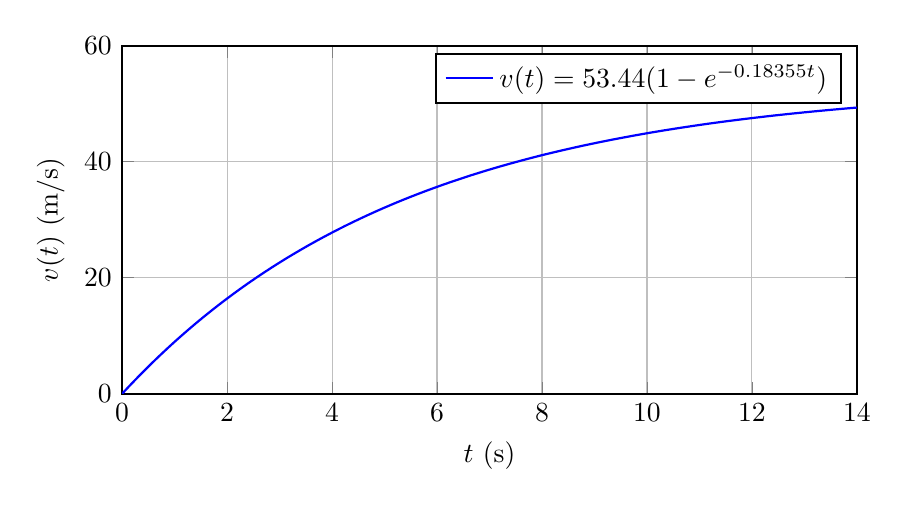
\begin{tikzpicture}
\begin{axis}[
  width=0.9\linewidth,
  height=6cm,
  xlabel={$t$ (s)},
  ylabel={$v(t)$ (m/s)},
  grid=major,
  ymin=0, ymax=60,
  xmin=0, xmax=14,
  samples=100,
  domain=0:14,
  thick
]
\addplot[blue, thick] {53.44*(1 - exp(-0.18355*x))};
\addlegendentry{$v(t) = 53.44(1 - e^{-0.18355t})$}
\end{axis}
\end{tikzpicture}
\end{frame}

%------------------------------
\begin{frame}[c]{Soluciones analíticas vs. numéricas}
%\footnotesize
\begin{block}{¿Qué ocurre si no hay solución exacta?}
\vspace{0.2cm}
Muchos modelos no pueden resolverse analíticamente. En estos casos, se aplican métodos numéricos que aproximan la solución mediante cálculos aritméticos.
\end{block}

\begin{block}{Ejemplo 1: derivada como cociente de diferencias}
\vspace{0.2cm}
\[
\frac{dv}{dt} \approx \frac{v_{i+1} - v_i}{t_{i+1} - t_i}
\]
\begin{itemize}
  \item Aproximación por diferencias finitas hacia adelante
  \item Es válida si \(\Delta t\) es pequeño
\end{itemize}
\end{block}
\end{frame}

\begin{frame}[c]{Método de Euler (forma explícita)}
%\footnotesize
\begin{block}{Aplicación de diferencias finitas}
\[
\frac{dv}{dt} = g - \frac{c}{m}v \Rightarrow
v_{i+1} = v_i + \left(g - \frac{c}{m}v_i\right)\Delta t
\]
\end{block}

\textbf{Interpretación:}
\begin{itemize}
  \item La pendiente \((g - \frac{c}{m}v_i)\) se calcula en cada paso
  \item Se multiplica por \(\Delta t\) y se suma al valor anterior
  \item Método iterativo para aproximar la solución paso a paso
\end{itemize}

\textbf{Forma general:}
\[
\text{valor nuevo} = \text{valor anterior} + \text{pendiente} \times \Delta t
\]
\end{frame}
\begin{frame}[c]{Ejemplo: Solución numérica del paracaidista}
%\footnotesize
\begin{block}{Planteamiento}
\vspace{0.2cm}
Resolver el mismo problema del Ejemplo  usando el método de Euler:
\[
v_{i+1} = v_i + \left(g - \frac{c}{m}v_i\right)\Delta t
\]
\begin{itemize}
  \item \( m = 68.1~\text{kg} \), \( c = 12.5~\text{kg/s} \), \( g = 9.81~\text{m/s}^2 \)
  \item Paso de tiempo: \( \Delta t = 2~\text{s} \)
  \item Condición inicial: \( v_0 = 0~\text{m/s} \)
\end{itemize}
\end{block}
\end{frame}

\begin{frame}[c]{Resultados del método de Euler}
%\footnotesize
\begin{columns}[T,onlytextwidth]
  \begin{column}{0.55\textwidth}
    \begin{block}{Velocidad numérica}
    \begin{tabular}{@{}rr@{}}
    \toprule
    \textbf{t (s)} & \textbf{v (m/s)} \\
    \midrule
    0  & 0.00 \\
    2  & 19.62 \\
    4  & 32.04 \\
    6  & 39.90 \\
    8  & 44.87 \\
    10 & 48.02 \\
    12 & 50.01 \\
    $\infty$ & 53.44 (vel. límite) \\
    \bottomrule
    \end{tabular}
    \end{block}
  \end{column}
  \begin{column}{0.42\textwidth}
    \begin{itemize}
      \item Se aproxima a la solución exacta
      \item Error reducido con pasos más pequeños
      \item Computacionalmente viable con software
    \end{itemize}
  \end{column}
\end{columns}
\end{frame}

\begin{frame}[c]{Comparación gráfica: solución exacta vs. numérica}
\centering
\footnotesize
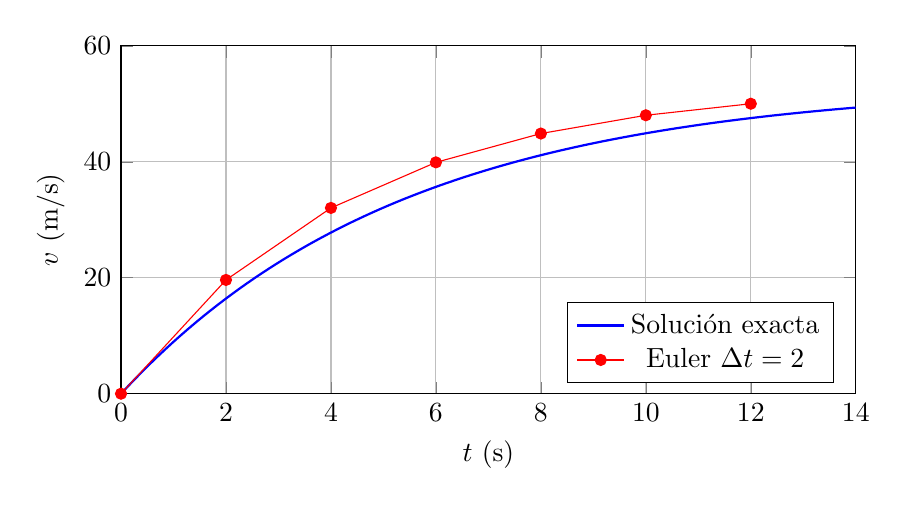
\begin{tikzpicture}
\begin{axis}[
  width=0.9\linewidth,
  height=6cm,
  xlabel={$t$ (s)},
  ylabel={$v$ (m/s)},
  grid=major,
  ymin=0, ymax=60,
  xmin=0, xmax=14,
  legend pos=south east
]
\addplot[blue, thick, domain=0:14, samples=100] {53.44*(1 - exp(-0.18355*x))};
\addlegendentry{Solución exacta}

\addplot[red, mark=*] coordinates {
  (0,0) (2,19.62) (4,32.04) (6,39.90) (8,44.87) (10,48.02) (12,50.01)
};
\addlegendentry{Euler $\Delta t = 2$}
\end{axis}
\end{tikzpicture}
\end{frame}



% ---- Diapositiva 1: Librerías y definición inicial
\begin{frame}[fragile]{Importación de librerías y función principal}
\begin{lstlisting}[style=mypython][style=mypython]
import numpy as np
import matplotlib.pyplot as plt

def euler_parachutist(m, c, g, dt, v0, t_final):
    """
    Resuelve la ecuación diferencial dv/dt = g - (c/m) * v
    mediante el método de Euler explícito.
    """
\end{lstlisting}
\end{frame}

% ---- Diapositiva 2: Desarrollo del método de Euler
\begin{frame}[fragile]{Desarrollo del método de Euler}
\begin{lstlisting}[style=mypython][style=mypython]
    n_steps = int(np.ceil(t_final / dt))
    t = np.linspace(0, n_steps * dt, n_steps + 1)
    v = np.zeros_like(t)
    v[0] = v0

    for i in range(n_steps):
        dvdt = g - (c / m) * v[i]
        v[i + 1] = v[i] + dvdt * dt

    return t, v
\end{lstlisting}
\end{frame}

% ---- Diapositiva 3: Función main - entrada de datos
\begin{frame}[fragile]{Función principal: entrada de datos}
\begin{lstlisting}[style=mypython]
def main():
    m = float(input("Masa m [kg]: "))
    c = float(input("Coeficiente de arrastre c [kg/s]: "))
    g_in = input("Gravedad g [m/s^2] (Enter = 9.81): ")
    g = float(g_in) if g_in else 9.81
    dt = float(input("Paso de tiempo dt [s]: "))
    v0 = float(input("Velocidad inicial v0 [m/s]: "))
    t_final = float(input("Tiempo final [s]: "))
\end{lstlisting}
\end{frame}

% ---- Diapositiva 4: Función main - resultados y gráfica
\begin{frame}[fragile]{Función principal: resultados y gráfica}
\begin{lstlisting}[style=mypython]
    t, v = euler_parachutist(m, c, g, dt, v0, t_final)

    print("\n  t (s)     v (m/s)")
    print("-" * 21)
    for ti, vi in zip(t, v):
        print(f"{ti:7.2f}   {vi:8.2f}")

    plt.plot(t, v, marker="o")
    plt.title("Velocidad del paracaidista (Euler)")
    plt.xlabel("t (s)")
    plt.ylabel("v (m/s)")
    plt.grid()
    plt.show()
\end{lstlisting}
\end{frame}

% ---- Diapositiva 5: Condición de ejecución
\begin{frame}[fragile]{Ejecución como programa principal}
\begin{lstlisting}[style=mypython]
if __name__ == "__main__":
    main()
\end{lstlisting}
\end{frame}



\begin{frame}[c]{Leyes de conservación e ingeniería}
%\footnotesize
\begin{block}{Principio general}
Muchas leyes fundamentales de la ingeniería pueden expresarse como:
\[
\text{Cambio} = \text{incremento} - \text{decremento} 
\]
Este formato se emplea para predecir cambios con el tiempo, por ejemplo, en el caso del paracaidista:
\[
\frac{dv}{dt} = \frac{mg - cv}{m}
\]
\end{block}

\begin{block}{Cálculo de variable-tiempo (transitorio)}
\medskip
Se usa cuando el \textbf{cambio no es cero}. Por ejemplo:
\begin{itemize}
  \item Velocidad cambiante del paracaidista
  \item Temperatura en un sistema térmico no estacionario
\end{itemize}
\end{block}
\end{frame}

\begin{frame}[c]{Estado estacionario y equilibrio}
%\footnotesize
\begin{block}{Cuando el cambio es cero}
\[
0 = \text{incremento} - \text{decremento} \Rightarrow \text{incremento} = \text{decremento}
\]
\textbf{Ejemplo:} flujo de fluido incompresible:
\[
\text{Flujo de entrada} = \text{flujo de salida}
\]
\end{block}

\begin{block}{Velocidad terminal del paracaidista (estado estacionario)}
\[
mg = cv \Rightarrow v = \frac{mg}{c}
\]
\begin{itemize}
  \item Fuerzas en equilibrio: gravedad = resistencia del aire
  \item \(v\): velocidad terminal
\end{itemize}
\end{block}
\end{frame}

\begin{frame}[c]{Importancia }
%\footnotesize
\begin{block}{Aplicaciones de ingeniería}
\begin{itemize}
  \item Cambios en tiempo: análisis transitorio.
  \item Sin cambios : análisis estacionario
  \item Ambas forman la base para modelar muchos procesos físicos
\end{itemize}
\end{block}

\begin{block}{Ejemplo destacado: balance de masa}
\begin{itemize}
  \item \textbf{Ley de conservación de la masa}
  \item Cambio de masa = entrada – salida
  \item Base del análisis en ingeniería química de reactores
\end{itemize}
\end{block}
\end{frame}

\subsection{Aproximaciones y errores de redondeo}
\begin{frame}[c]{Aproximaciones y errores de redondeo}
%\footnotesize
\begin{itemize}
  \item Los métodos numéricos entregan soluciones \textbf{aproximadas}, no exactas.
  \item Se generan \textbf{errores} por distintas causas:
  \begin{itemize}
    \item Redondeo: debido a que la computadora usa un número finito de dígitos.
    \item Truncamiento: cuando se utilizan aproximaciones en lugar de operaciones exactas.
    \item Modelado o datos: errores en la formulación o incertidumbre en los datos.
  \end{itemize}
  \item En muchos casos, \textbf{no existe una solución analítica} para comparar, por lo que se requiere estimar el error.
  \item Es importante \textbf{cuantificar y minimizar} estos errores para garantizar la fiabilidad del resultado numérico.
  \item La \textbf{tolerancia al error} dependerá del contexto ingenieril: no siempre se necesita exactitud total.
\end{itemize}
\end{frame}

\begin{frame}[c]{Cifras significativas y error de redondeo}
\footnotesize
\begin{columns}[T,onlytextwidth]
  \begin{column}{0.6\textwidth}
    \begin{itemize}
      \item Los métodos numéricos producen resultados \textbf{aproximados}, por lo tanto se necesita un criterio de confiabilidad.
      \item Uno de ellos es el número de \textbf{cifras significativas} correctas.
      \item Ejemplo: un resultado es aceptable si es correcto a 4 cifras significativas.
      \item Números como \(\pi,\ e\) o fracciones como \(\frac{7}{3}\) no pueden representarse exactamente con un número finito de dígitos.
      \item La diferencia entre la cantidad real y su representación finita se denomina \textbf{error de redondeo}.
      \item El concepto de cifras significativas será clave para definir \textbf{exactitud y precisión} en los cálculos numéricos.
    \end{itemize}
  \end{column}
  \begin{column}{0.4\textwidth}
    \centering
    
\includegraphics[width=0.95\textwidth]{Numerical_Methods/img/ejemplifican_concepto_cifras_significativas.png}\\[0.5ex]
    \scriptsize Ejemplo de lectura con redondeo e incertidumbre visual
  \end{column}
\end{columns}
\end{frame}

\begin{frame}{exactitud y precisión }
    \begin{figure}
        \centering
        
\includegraphics[width=0.48\linewidth]{Numerical_Methods/img/exac_precision.png}
        \caption{Conceptos de exactitud y precisión}
        \label{fig:enter-label}
    \end{figure}
\end{frame}


\begin{frame}[c]{Errores en métodos numéricos}
%\footnotesize
\begin{itemize}
  \item Los errores surgen por aproximar operaciones exactas:
  \begin{itemize}
    \item \textbf{Truncamiento}: aproximar un proceso matemático exacto.
    \item \textbf{Redondeo}: representar números con cifras significativas limitadas.
  \end{itemize}
  \item Relación general:
  \[
\boxed{\text{Valor verdadero} = \text{valor aproximado} + \text{error}}
  \]
  \item Error verdadero:
  \[
\boxed{ E_t = \text{valor verdadero} - \text{valor aproximado}}
  \]
\end{itemize}
\begin{itemize}
  \item Se normaliza el error respecto al valor verdadero:
  \[
\boxed{\varepsilon_t = \frac{\text{valor verdadero} - \text{valor aproximado}}{\text{valor verdadero}} \times 100\%}\]
  \item\(\varepsilon_t\) denota el error relativo porcentual verdadero.
\end{itemize}
\end{frame}

\begin{frame}[c]{Ejemplo: Cálculo de errores}
\footnotesize
\begin{block}{Puente vs. remache}
Suponga que se tiene que medir la longitud de un puente y la de
un remache, y se obtiene 9 999 y 9 cm, respectivamente. Si los valores verdaderos son 10 000 y 10 cm, calcule 
a) el error verdadero y b) el error relativo porcentual verdadero en cada caso.
\begin{itemize}
  \item Longitudes medidas: 9 999 cm (puente), 9 cm (remache)
  \item Valores reales: 10 000 cm y 10 cm
\end{itemize}
\textbf{a) Error verdadero:}
\[
E_t = 10\,000 - 9\,999 = 1~\text{cm}, \quad E_t = 10 - 9 = 1~\text{cm}
\]
\textbf{b) Error relativo porcentual:}
\[
\frac{1}{10\,000} \times 100 = 0.01\% \quad \text{(puente)}
\quad \frac{1}{10} \times 100 = 10\% \quad \text{(remache)}
\]
\end{block}
\end{frame}

\begin{frame}[c]{Error relativo porcentual aproximado}
%\footnotesize
\begin{itemize}
  \item En problemas reales, el valor verdadero no siempre es conocido.
  \item Se estima el error relativo con respecto a la mejor aproximación:
  \[
\boxed{  \varepsilon_a = \frac{\text{error aproximado}}{\text{valor aproximado}} \times 100\%}
  \]
  \item En métodos iterativos:
  \[
\boxed{\varepsilon_a = \frac{|x_{\text{actual}} - x_{\text{anterior}}|}{|x_{\text{actual}}|} \times 100\%}
  \]
\end{itemize}
\end{frame}

\begin{frame}[c]{Criterio de tolerancia y cifras significativas}
%\footnotesize
\begin{itemize}
  \item Se detiene la iteración cuando:
  \[
\boxed{  |\varepsilon_a| < \varepsilon_s}
  \]
  \item Se relaciona la tolerancia con cifras significativas:
  \[
  \boxed{ \varepsilon_s = 0.5 \times 10^{2 - n}\%} \quad \text{(Scarborough, 1966)}
  \]
  \item Donde:
  \begin{itemize}
    \item \(\varepsilon_s\): error tolerado en porcentaje
    \item \(n\): número de cifras significativas deseadas
  \end{itemize}
\end{itemize}
\end{frame}

\begin{frame}[c]{Ejemplo:  Estimación del error iterativo}
%\footnotesize
\begin{block}{Planteamiento}
\begin{itemize}
  \item Se desea calcular \( e^{0.5} \approx 1.648721\) usando su serie de Maclaurin:
  \[
  e^x = 1 + x + \frac{x^2}{2!} + \frac{x^3}{3!} + \dots + \frac{x^n}{n!}
  \]
  \item Se agregan términos uno a uno, hasta que el error relativo aproximado \(\varepsilon_a < 0.05\%\) (3 cifras significativas).
\end{itemize}
\end{block}
\end{frame}

\begin{frame}[c]{Paso 1: Primeros términos}
%\footnotesize
\textbf{Término 1:} \( e^x = 1 \Rightarrow \)
\[
  \varepsilon_t = \frac{1.648721 - 1}{1.648721} \times 100 \approx 39.3\% \quad \text{(error verdadero)}
\]
\textbf{Término 2:} \( e^x = 1 + 0.5 = 1.5 \Rightarrow \)
\begin{align*}
  \varepsilon_t &= \frac{1.648721 - 1.5}{1.648721} \times 100 \approx 9.02\% \\
  \varepsilon_a &= \frac{1.5 - 1}{1.5} \times 100 \approx 33.3\%
\end{align*}
\end{frame}

\begin{frame}[c]{Paso 2: Término 3 y 4}
%\footnotesize
\textbf{Término 3:} \( 1 + 0.5 + \frac{0.5^2}{2!} = 1.625 \)
\begin{align*}
  \varepsilon_t &= \frac{1.648721 - 1.625}{1.648721} \times 100 \approx 1.44\% \\
  \varepsilon_a &= \frac{1.625 - 1.5}{1.625} \times 100 \approx 7.69\%
\end{align*}

\textbf{Término 4:} \( 1.625 + \frac{0.5^3}{3!} = 1.645833... \)
\begin{align*}
  \varepsilon_t &\approx 0.22\% \\
  \varepsilon_a &\approx 1.21\%
\end{align*}
\end{frame}

\begin{frame}[c]{Paso 3: Término 5 y 6}
%\footnotesize
\textbf{Término 5:} \( 1.645833 + \frac{0.5^4}{4!} = 1.647604 \)
\begin{align*}
  \varepsilon_t &\approx 0.01\% \\
  \varepsilon_a &\approx 0.12\%
\end{align*}

\textbf{Término 6:} \( 1.648438 + \frac{0.5^5}{5!} = 1.64786 \)
\begin{align*}
  \varepsilon_t &\approx 0.052\% \\
  \varepsilon_a &\approx 0.015\% < 0.05\% \Rightarrow \textbf{criterio cumplido}
\end{align*}
\end{frame}

\begin{frame}[c]{Resumen de iteraciones}
\footnotesize
\begin{tabular}{@{}cccc@{}}
\toprule

\textbf{Términos} & \textbf{Resultado} & \(\varepsilon_t\, (\%)\) & \(\varepsilon_a\, (\%)\) \\
\midrule
1 & 1.000000 & 39.3  & --- \\
2 & 1.500000 & 9.02  & 33.3 \\
3 & 1.625000 & 1.44  & 7.69 \\
4 & 1.645833 & 0.175 & 1.27 \\
5 & 1.648438 & 0.0172 & 0.158 \\
6 & 1.648698 & 0.00142 & 0.0158 \\
\bottomrule
\end{tabular}

\vspace{1ex}
\textbf{Conclusión:} Se requiere un total de 6 términos para garantizar al menos 3 cifras significativas con \(\varepsilon_s = 0.05\%\).
\end{frame}


% ---------- Diapositiva 1: Entrada simulada y función ----------
\begin{frame}[fragile]{Definición de función y entrada de datos}

\begin{lstlisting}[style=mypython]
import math

def estimar_exponencial(x, tolerancia_percent):
    valor_real = math.exp(x)  # Valor verdadero de e^x
    estimacion = 1.0          # primer término: x^0 / 0! = 1
    termino = 1.0             # valor del término actual
    n = 1
    errores = []

    et = abs((valor_real - estimacion) / valor_real) * 100
    errores.append((0, estimacion, None, et))  # Paso inicial (n=0)


\end{lstlisting}
\end{frame}

% ---------- Diapositiva 3: Cálculo y simulación de entrada ----------
\begin{frame}[fragile]{Cálculo iterativo y errores}
\begin{lstlisting}[style=mypython]
     while True:
        termino *= x / n
        nueva_estimacion = estimacion + termino
        ea = abs((termino / nueva_estimacion) * 100)           # error relativo aproximado
        et = abs((valor_real - nueva_estimacion) / valor_real) * 100  # error verdadero
        errores.append((n, nueva_estimacion, ea, et))

        if ea < tolerancia_percent:
            break

        estimacion = nueva_estimacion
        n += 1

    return nueva_estimacion, errores, valor_real

\end{lstlisting}
\end{frame}

% ---------- Diapositiva 3: Cálculo y simulación de entrada ----------
\begin{frame}[fragile]{Cálculo iterativo y errores}
\begin{lstlisting}[style=mypython]
# ---- Entrada de datos interactiva ----
print("Estimación de e^x usando la serie de Maclaurin")
x = float(input("Ingrese el valor de x: "))
tol = float(input("Ingrese la tolerancia de error relativo (%) (ej: 0.05): "))
# ---- Cálculo y salida ----
aprox_final, pasos, real = estimar_exponencial(x, tol)

print(f"\nValor real: e^{x} ≈ {real:.8f}")
print(f"Aproximación final: {aprox_final:.8f}")
print("\nIteraciones:")
print(" n   estimación       εa (%)     εt (%)")
print("-" * 45)
for n, val, ea, et in pasos:
    ea_str = "---     0.5" if ea is None else f"{ea:8.5f}"
    print(f"{n:2d}   {val:.8f}   {ea_str}   {et:8.5f}")

\end{lstlisting}
\end{frame}


\subsection{Errores de truncamiento y la serie de Taylor}

\begin{frame}{Errores de truncamiento}
%\footnotesize
\begin{itemize}
  \item Surgen al usar una \textbf{aproximación} en lugar de un procedimiento exacto.
  \item Ejemplo: aproximación de derivadas con diferencias finitas.
  \item Son inevitables en los métodos numéricos.
  \item Para analizarlos se usa la \textbf{serie de Taylor}.
\end{itemize}

\begin{block}{Propósito}
Permite predecir el valor de una función en un punto, usando su valor y derivadas en otro punto.
\end{block}
\begin{itemize}
  \item \( f(x_{i+1}) \approx f(x_i) \) — orden 0
  \item \( f(x_{i+1}) \approx f(x_i) + f'(x_i)(x_{i+1} - x_i) \) — orden 1
  \item \( f(x_{i+1}) \approx f(x_i) + f'(x_i)h + \frac{f''(x_i)}{2!}h^2 \) — orden 2
\end{itemize}
\end{frame}

\begin{frame}{Serie completa de Taylor}
%\footnotesize
\begin{equation*}
\boxed{  f(x_{i+1}) = f(x_i) + f'(x_i)h + \frac{f''(x_i)}{2!}h^2 + \dots + \frac{f^{(n)}(x_i)}{n!}h^n + R_n}
\end{equation*}
\begin{itemize}
  \item \( h = x_{i+1} - x_i \)
  \item \( R_n \) es el término residual (error de truncamiento)
  \item La serie es infinita; truncarla genera el error.
\end{itemize}
\end{frame}

\begin{frame}{Teorema de Taylor}
\small
\begin{block}{Idea general}
\vspace{0.2cm}
El Teorema de Taylor permite aproximar una función suave mediante
un polinomio construido a partir de sus derivadas en un punto.
\end{block}

\begin{itemize}
  \item Si \(f\) y sus derivadas hasta orden \(n+1\) son continuas en un intervalo que contiene \(a\) y \(x\),
  entonces:
\[
f(x) = f(a) 
+ f'(a)(x-a)
+ \frac{f''(a)}{2!}(x-a)^2
+ \cdots
+ \frac{f^{(n)}(a)}{n!}(x-a)^n
+ R_n
\]
  \item Esta expansión se conoce como \textbf{Serie de Taylor}.
  \item \(R_n\) es el residuo o \textbf{error de truncamiento}.
\end{itemize}
\end{frame}

\begin{frame}{Forma integral del residuo}
\small
\begin{block}{Residuo en forma integral}
\[
R_n = \int_{a}^{x} 
\frac{f^{(n+1)}(t)}{n!}
(x-t)^n\, dt
\]
\end{block}

\begin{itemize}
  \item Esta expresión se obtiene integrando repetidamente por partes.
  \item \(t\) es una variable muda de integración.
  \item El término mide la diferencia entre la función real y su polinomio de Taylor.
  \item Para avanzar hacia la forma de Lagrange, se necesita el \textbf{Teorema del Valor Medio}.
\end{itemize}
\end{frame}

\begin{frame}{Primer Teorema del Valor Medio para integrales}
\small
\begin{block}{Enunciado}
Si \(g(t)\) es continua en un intervalo que contiene \(a\) y \(x\), entonces existe
\(\xi \in (a,x)\) tal que:
\[
\int_a^x g(t)\, dt = g(\xi)(x-a)
\]
\end{block}

\begin{itemize}
  \item La integral se puede interpretar como el “promedio” de la función
    multiplicado por la longitud del intervalo.
  \item La función necesariamente alcanza ese valor promedio en algún punto.
\end{itemize}
\end{frame}
\begin{frame}{Segundo Teorema del Valor Medio para integrales}
\small
\begin{block}{Enunciado}
Si \(g\) y \(h\) son continuas en un intervalo que contiene \(a\) y \(x\), 
y \(h(t)\) no cambia de signo, entonces:
\[
\int_a^x g(t)h(t)\,dt = g(\xi)\int_a^x h(t)\, dt
\]
para algún \(\xi \in (a,x)\).
\end{block}

\begin{itemize}
  \item El primer teorema es un caso especial donde \(h(t)=1\).
  \item Esta versión permite manejar integrandos de la forma \(g(t)h(t)\).
\end{itemize}
\end{frame}
\begin{frame}{Aplicación del Teorema del Valor Medio al residuo}
\small

\[
R_n = \int_{a}^{x} 
\frac{f^{(n+1)}(t)}{n!} (x-t)^n\, dt
\]

Tomamos:
\[
g(t) = f^{(n+1)}(t), \qquad
h(t) = \frac{(x-t)^n}{n!}
\]

\begin{itemize}
  \item \(h(t)\) es continua y no cambia de signo en \([a,x]\).
  \item Por el Segundo Teorema del Valor Medio:
\[
R_n = f^{(n+1)}(\xi)
\int_{a}^{x} \frac{(x-t)^n}{n!}\, dt
\]
\end{itemize}
\end{frame}
\begin{frame}{Cálculo de la integral del residuo}
\small

\[
\int_{a}^{x} \frac{(x-t)^n}{n!}\, dt
\]

Hacemos el cambio de variable \(u = x-t\):

\[
\int_{0}^{x-a} \frac{u^n}{n!}\, du
= \frac{1}{n!}\left[\frac{u^{n+1}}{n+1}\right]_{0}^{x-a}
\]

\[
= \frac{(x-a)^{n+1}}{(n+1)!}
\]

\begin{block}{Sustituyendo en la expresión de \(R_n\)}
\[
R_n = \frac{f^{(n+1)}(\xi)}{(n+1)!}(x-a)^{n+1}
\]
\end{block}
\end{frame}
\begin{frame}{Forma de Lagrange del residuo}
\small
\begin{block}{Resultado final}
\[
\boxed{
R_n = \frac{f^{(n+1)}(\xi)}{(n+1)!}(x-a)^{n+1}
}
\quad\text{para algún } \xi\in(a,x)
\]
\end{block}

\begin{itemize}
  \item Esta es la \textbf{forma de Lagrange} del residuo.
  \item Permite estimar el error de truncamiento sin evaluar la serie completa.
  \item Garantiza que el polinomio de Taylor aproxima a la función con precisión controlable.
\end{itemize}
\end{frame}



\begin{frame}{Ejemplo 5 Aproximación de un polinomio}
%\footnotesize
\textbf{Función:} \(f(x) = -0.1x^4 - 0.15x^3 - 0.5x^2 - 0.25x + 1.2\)
\begin{itemize}
  \item Aproximar \(f(1)\) usando la serie de Taylor centrada en \(x = 0\)
  \item Valor exacto: \(f(1) = 0.2\)
\end{itemize}

%\footnotesize
\[
  f(1) \approx f(0) = 1.2
\]
\textbf{Error de truncamiento:} \(E_t = 0.2 - 1.2 = -1.0\)


\[
  f'(x) = -0.4x^3 - 0.45x^2 - x - 0.25 \Rightarrow f'(0) = -0.25
\]
\[
  f(1) \approx f(0) + f'(0)(1) = 1.2 - 0.25 = 0.95
\]
\textbf{Error:} \(E_t = 0.2 - 0.95 = -0.75\)
\end{frame}

\begin{frame}{Orden 2: parábola}
%\footnotesize
\[
  f''(x) = -1.2x^2 - 0.9x - 1 \Rightarrow f''(0) = -1
\]
\[
  f(1) \approx 1.2 - 0.25 - 0.5 = 0.45
\]
\textbf{Error:} \(E_t = 0.2 - 0.45 = -0.25\)
\[
  f(1) = 1.2 - 0.25(1) - 0.5(1)^2 - 0.15(1)^3 - 0.1(1)^4 = 0.2
\]
\begin{itemize}
  \item El resultado coincide con el valor exacto
  \item El residuo de orden 5 es cero porque la derivada quinta de un polinomio de grado 4 es cero
\end{itemize}
\end{frame}

\begin{frame}{Ejemplo 5: Aproximación de Taylor - Solución Gráfica}

% Columna izquierda: Gráfico
\vspace*{0cm}
\centering
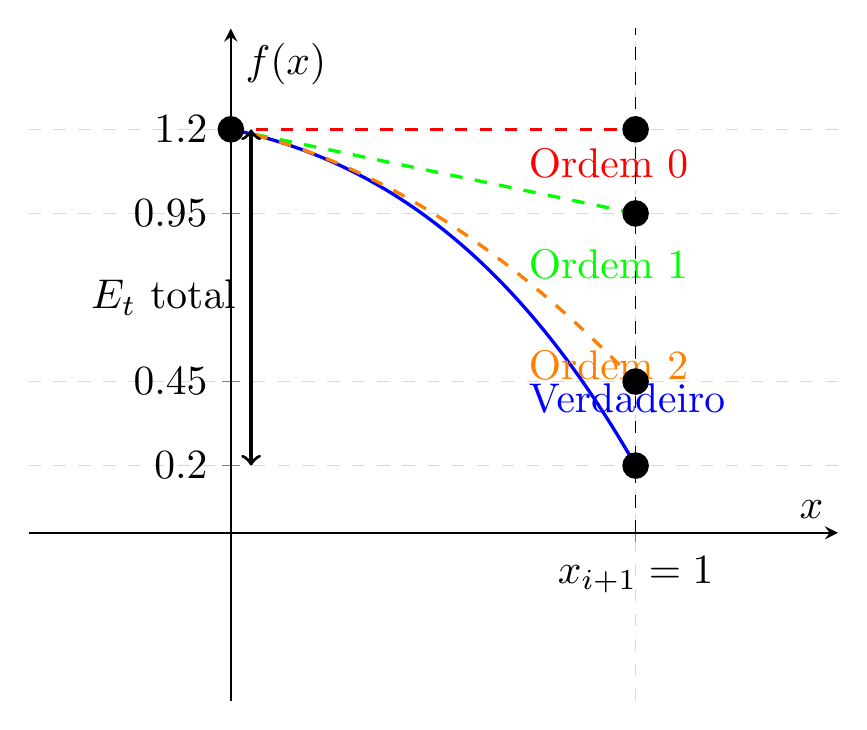
\begin{tikzpicture}[scale=1.5]
\begin{axis}[
    axis lines = middle,
    xlabel = $x$,
    ylabel = $f(x)$,
    xmin=-0.5, xmax=1.5,
    ymin=-0.5, ymax=1.5,
    xtick={-1,1},
    xticklabels={$x_i=0$,$x_{i+1}=1$},
    ytick={0,0.2,0.45,0.95,1.2},
    yticklabels={0,0.2,0.45,0.95,1.2},
    grid=major,
    grid style={dashed,gray!30},
]

% Función verdadera
\addplot [
    domain=0:1,
    samples=100,
    color=blue,
    thick
] {-0.1*x^4 - 0.15*x^3 - 0.5*x^2 - 0.25*x + 1.2};
\node at (0.7,0.4) [anchor=west, blue] {Verdadeiro};

% Orden 0 (constante)
\addplot [
    domain=0:1,
    samples=2,
    color=red,
    thick,
    dashed
] {1.2};
\node at (0.7,1.1) [anchor=west, red] {Ordem 0};

% Orden 1 (lineal)
\addplot [
    domain=0:1,
    samples=2,
    color=green,
    thick,
    dashed
] {1.2 - 0.25*x};
\node at (0.7,0.8) [anchor=west, green] {Ordem 1};

% Orden 2 (parabólica)
\addplot [
    domain=0:1,
    samples=100,
    color=orange,
    thick,
    dashed
] {1.2 - 0.25*x - 0.5*x^2};
\node at (0.7,0.5) [anchor=west, orange] {Ordem 2};

% Puntos importantes
\addplot[only marks, mark=*, mark size=3pt] coordinates {
    (0,1.2)
    (1,0.2)
    (1,1.2)
    (1,0.95)
    (1,0.45)
};

% Líneas verticales
\draw[dashed] (1,0) -- (1,1.5);
\draw[<->, thick] (0.05,1.2) -- (0.05,0.2) node[midway,left] {$E_t$ total};
\end{axis}
\end{tikzpicture}

\end{frame}

\begin{frame}{Serie de Taylor: Exactitud y Error de Truncamiento}
\begin{block}{Exactitud para polinomios}
\begin{itemize}
\item La expansión de Taylor de orden $n$ es \alert{exacta} para polinomios de grado $n$
\item Para funciones no polinomiales (exponenciales, senoidales), se requiere \alert{infinitos términos} para obtener el valor exacto
\end{itemize}
\end{block}

\begin{block}{Error de truncamiento}
\[ R_n = \frac{f^{(n+1)}(\xi)}{(n+1)!}h^{n+1} \quad \text{con} \quad \xi \in (x_i, x_{i+1}) \]
\begin{itemize}
\item \alert{Dilema}: Requiere conocer $f^{(n+1)}(x)$ (pero si se conoce $f(x)$, no se necesitaría la aproximación)
\item Notación $R_n=O(h^{n+1})$ indica que el error es proporcional a $h^{n+1}$
\end{itemize}
\end{block}
\end{frame}

\begin{frame}{Comportamiento del error}
\begin{tabular}{lcc}
\toprule
\textbf{Orden del error} & \textbf{Reducción de $h$} & \textbf{Reducción del error} \\
\midrule
$O(h)$ & $h \to h/2$ & Error $\to$ Error/2 \\
$O(h^2)$ & $h \to h/2$ & Error $\to$ Error/4 \\
$O(h^3)$ & $h \to h/2$ & Error $\to$ Error/8 \\
\bottomrule
\end{tabular}


\begin{alertblock}{Conclusión}
\begin{itemize}
\item Pocos términos pueden dar aproximaciones \alert{suficientemente buenas} para aplicaciones prácticas
\item La elección del orden depende del balance entre \alert{precisión requerida} y \alert{complejidad computacional}
\end{itemize}
\end{alertblock}
\end{frame}

\begin{frame}{Ejemplo 6: Planteamiento del problema}
%\footnotesize
\begin{block}{Objetivo}
Aproximar $f\left(\frac{\pi}{3}\right) = \cos\left(\frac{\pi}{3}\right) = 0.5$ usando la serie de Taylor centrada en $x_i = \frac{\pi}{4}$ ($h = \frac{\pi}{12}$)
\end{block}

\begin{columns}[T]
\column{0.5\textwidth}
\textbf{Datos:}
\begin{itemize}
\item $f(x) = \cos x$
\item $x_i = \frac{\pi}{4}$
\item $x_{i+1} = \frac{\pi}{3}$
\item $h = \frac{\pi}{3} - \frac{\pi}{4} = \frac{\pi}{12}$
\end{itemize}

\column{0.5\textwidth}
\textbf{Derivadas:}
\begin{align*}
f(x) &= \cos x \\
f'(x) &= -\sin x \\
f''(x) &= -\cos x \\
f'''(x) &= \sin x \\
f^{(4)}(x) &= \cos x \\
&\vdots
\end{align*}
\end{columns}
\end{frame}

\begin{frame}{Aproximaciones de orden 0 a 2}
\begin{columns}[T]
\column{0.5\textwidth}
\begin{block}{Orden 0}
\[ f\left(\frac{\pi}{3}\right) \approx \cos\left(\frac{\pi}{4}\right) = 0.707106781 \]
\[ \varepsilon_t = -41.4\% \]
\end{block}

\begin{block}{Orden 1}
\[ f\left(\frac{\pi}{3}\right) \approx \cos\left(\frac{\pi}{4}\right) - \sin\left(\frac{\pi}{4}\right)\left(\frac{\pi}{12}\right) \]
\[ = 0.521986659 \]
\[ \varepsilon_t = -4.40\% \]
\end{block}

\column{0.5\textwidth}
\begin{block}{Orden 2}
\[ f\left(\frac{\pi}{3}\right) \approx \cos\left(\frac{\pi}{4}\right) - \sin\left(\frac{\pi}{4}\right)\left(\frac{\pi}{12}\right) \]
\[ - \frac{\cos\left(\frac{\pi}{4}\right)}{2!}\left(\frac{\pi}{12}\right)^2 \]
\[ = 0.497754491 \]
\[ \varepsilon_t = 0.449\% \]
\end{block}
\end{columns}
\end{frame}

\begin{frame}{Aproximaciones de orden 3 a 6}
\begin{columns}[T]
\column{0.5\textwidth}
\begin{block}{Orden 3}
\[ +\frac{\sin\left(\frac{\pi}{4}\right)}{3!}\left(\frac{\pi}{12}\right)^3 \]
\[ = 0.499869147 \]
\[ \varepsilon_t = 2.62 \times 10^{-2}\% \]
\end{block}

\begin{block}{Orden 4}
\[ +\frac{\cos\left(\frac{\pi}{4}\right)}{4!}\left(\frac{\pi}{12}\right)^4 \]
\[ = 0.500007551 \]
\[ \varepsilon_t = -1.51 \times 10^{-3}\% \]
\end{block}

\column{0.5\textwidth}
\begin{block}{Orden 5}
\[ -\frac{\sin\left(\frac{\pi}{4}\right)}{5!}\left(\frac{\pi}{12}\right)^5 \]
\[ = 0.500000304 \]
\[ \varepsilon_t = -6.08 \times 10^{-5}\% \]
\end{block}

\begin{block}{Orden 6}
\[ -\frac{\cos\left(\frac{\pi}{4}\right)}{6!}\left(\frac{\pi}{12}\right)^6 \]
\[ = 0.499999988 \]
\[ \varepsilon_t = 2.40 \times 10^{-6}\% \]
\end{block}
\end{columns}
\end{frame}

\begin{frame}{Resumen de resultados}
\centering
\footnotesize
\begin{tabular}{cccc}
\toprule
\textbf{Orden (n)} & \textbf{Aproximación} & \textbf{Error (\%)} & \textbf{Mejora} \\
\midrule
0 & 0.707106781 & -41.4 & -- \\
1 & 0.521986659 & -4.40 & 10$\times$ \\
2 & 0.497754491 & 0.449 & 10$\times$ \\
3 & 0.499869147 & $2.62 \times 10^{-2}$ & 17$\times$ \\
4 & 0.500007551 & $-1.51 \times 10^{-3}$ & 17$\times$ \\
5 & 0.500000304 & $-6.08 \times 10^{-5}$ & 25$\times$ \\
6 & 0.499999988 & $2.40 \times 10^{-6}$ & 25$\times$ \\
\bottomrule
\end{tabular}

\begin{block}{Observaciones clave}
\begin{itemize}
\item Cada término adicional mejora la aproximación
\item La mayor mejora relativa ocurre en los primeros órdenes
\item Con 6 términos se alcanza error $< 0.000003\%$
\item La serie converge pero nunca se hace exacta (requeriría infinitos términos)
\end{itemize}
\end{block}
\end{frame}


% ---------- Diapositiva 1: Entrada simulada y función ----------
\begin{frame}[fragile]{Definición de función y entrada de datos}

\begin{lstlisting}[style=mypython]
import math
import pandas as pd
from math import pi

def cos_maclaurin_aprox(x, tolerancia_percent):
    valor_real = math.cos(x)
    suma = 0.0
    n = 0
    errores = []


\end{lstlisting}
\end{frame}

% ---------- Diapositiva 3: Cálculo y simulación de entrada ----------
\begin{frame}[fragile]{Cálculo iterativo y errores}
\begin{lstlisting}[style=mypython]
     while True:
        signo = (-1) ** n
        termino = signo * (x ** (2 * n)) / math.factorial(2 * n)
        suma_nueva = suma + termino
        et = abs((valor_real - suma_nueva) / valor_real) * 100
        if n == 0:
            ea = None
        else:
            ea = abs(termino / suma_nueva) * 100
        errores.append((n, termino, suma_nueva, ea, et))
        if ea is not None and ea < tolerancia_percent:
            break
        suma = suma_nueva
        n += 1
    return errores
\end{lstlisting}
\end{frame}

% ---------- Diapositiva 3: Cálculo y simulación de entrada ----------
\begin{frame}[fragile]{Cálculo iterativo y errores}
\begin{lstlisting}[style=mypython]
# --- Entrada de datos desde el usuario ---
print("Aproximación de cos(x) usando la serie de Maclaurin")
x = eval(input("Ingrese x en radianes (puede usar pi, ej: pi/3): "))
tol = float(input("Ingrese la tolerancia de error relativo (%) (ej: 5): "))

resultados = cos_maclaurin_aprox(x, tol)

# --- Mostrar tabla de resultados ---
print("\nResultados:")
print(" n   Término        Aproximación     εa (%)       εt (%)")
print("-" * 60)
for n, term, aprox, ea, et in resultados:
    ea_str = "---    " if ea is None else f"{ea:10.5f}"
    print(f"{n:<2}  {term:12.6f}   {aprox:14.6f}   {ea_str:>8}   {et:10.5f}")
\end{lstlisting}
\end{frame}


%------------------------------------------------------------
\begin{frame}{Teorema de Taylor y término de resto}
\small          % texto ligeramente más compacto

\begin{columns}[c]

% ---------- Columna de la explicación ----------------------
\column{0.58\textwidth}

Sea \(h = x_{i+1}-x_i\). El desarrollo de Taylor hasta el término lineal y su resto es
\[
f(x_i+h)\;=\;f(x_i) \;+\; f'(x_i)\,h \;+\; R_0,
\]
donde, aplicando el teorema del valor medio,
\[
\boxed{\,R_0 \;=\; f'(\xi_0)\,h\,,\qquad \xi_0\in(x_i,x_{i+1})}
\]

\medskip
\textbf{Extensión: resto de primer orden}
\[
f(x_i+h)\;=\;f(x_i)+f'(x_i)\,h+\frac{f''(x_i)}{2!}\,h^{2}+R_1,
\]
con
\[
\boxed{\,R_1 \;=\; \dfrac{f''(\xi_1)}{2!}\,h^{2}\,,\qquad \xi_1\in(x_i,x_{i+1})}
\]

\medskip
Los términos de orden superior (\(R_2, R_3,\dots\)) se obtienen iterando el mismo
razonamiento sobre derivadas sucesivas.

% ---------- Columna de la figura ---------------------------
\column{0.42\textwidth}
\centering

\includegraphics[width=\linewidth]{Numerical_Methods/img/residui de orden cero.png}\\[0.3em]
\footnotesize Representación gráfica del residuo de orden cero

\end{columns}
\end{frame}
%------------------------------------------------------------

%------------------------------------------------------------
\begin{frame}{Serie de Taylor y error de truncamiento}
\small

\begin{columns}[c]

%-------------- Columna A: desarrollo teórico -------------------
\column{0.6\textwidth}

\begin{block}{Expansión de \(v(t)\) alrededor de \(t_i\)}
\[
v(t_{i+1}) = v(t_i)
           + v'(t_i)\,\Delta t
           + \frac{v''(t_i)}{2!}\,\Delta t^2 + \cdots + R_n
\]
\end{block}
\footnotesize
Truncando después del término lineal:
\[
v(t_{i+1}) = v(t_i) + v'(t_i)\,\Delta t + R_1
\]

\[
\boxed{\,v'(t_i) \;\approx\;
       \dfrac{v(t_{i+1})-v(t_i)}{\Delta t}\,}
\quad\text{con}\quad
R_1 = -\dfrac{v''(\xi_1)}{2!}\,\Delta t
\]

\[
|R_1| = \mathcal{O}\!\bigl(\,\Delta t\,\bigr)
\]

\medskip
\footnotesize
Reducir \(\Delta t\) a la mitad también reduce a la mitad el error de truncamiento.

%-------------- Columna B: imagen --------------------------------
\column{0.4\textwidth}
\centering

\includegraphics[width=\linewidth]{Numerical_Methods/img/valor medio .png}\\[0.3em]
\footnotesize
Representación gráfica del error de truncamiento
% Cambia "img/error_truncamiento.png" por la ruta a tu archivo

\end{columns}
\end{frame}
%------------------------------------------------------------




\begin{frame}{Comparación de residuos}
\centering
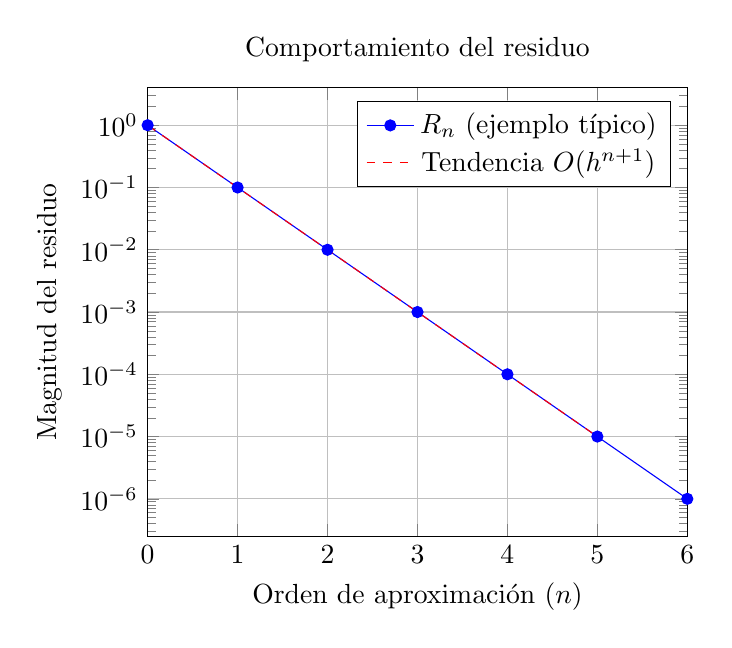
\begin{tikzpicture}
\begin{axis}[
    title={Comportamiento del residuo},
    xlabel={Orden de aproximación ($n$)},
    ylabel={Magnitud del residuo},
    ymin=0,
    xmin=0, xmax=6,
    xtick={0,1,2,3,4,5,6},
    grid=major,
    legend pos=north east,
    ymode=log
]

\addplot[blue, mark=*] coordinates {
    (0, 1)
    (1, 0.1)
    (2, 0.01)
    (3, 0.001)
    (4, 0.0001)
    (5, 0.00001)
    (6, 0.000001)
};
\addlegendentry{$R_n$ (ejemplo típico)}

\addplot[red, dashed] {10^(-x)};
\addlegendentry{Tendencia $O(h^{n+1})$}
\end{axis}
\end{tikzpicture}

\begin{block}{Observación clave}
\[ R_n = O(h^{n+1}) \]
\begin{itemize}
\item El error disminuye rápidamente al aumentar el orden
\item Para $h < 1$, términos superiores contribuyen menos
\end{itemize}
\end{block}
\end{frame}

%------------------------------------------------------------
%------------------------------------------------------------
\subsection{Diferenciación numérica: diferencias finitas}
\begin{frame}{Diferenciación numérica: diferencias finitas}
\small

\begin{columns}[c]

%----------------- Columna A: contenido teórico -------------------
\column{0.60\textwidth}

\textbf{Primera derivada mediante:}

\medskip
\textbf{• Diferencia hacia adelante (orden \(O(h)\))}  
\[
f'(x_i) \approx \frac{f(x_{i+1}) - f(x_i)}{h}
\quad \text{con error } \mathcal{O}(h)
\]

\textbf{• Diferencia hacia atrás (orden \(O(h)\))}  
\[
f'(x_i) \approx \frac{f(x_i) - f(x_{i-1})}{h}
\quad \text{con error } \mathcal{O}(h)
\]

\textbf{• Diferencia centrada (orden \(O(h^2)\))}  
\[
f'(x_i) \approx \frac{f(x_{i+1}) - f(x_{i-1})}{2h}
\quad \text{con error } \mathcal{O}(h^2)
\]



%----------------- Columna B: imagen -------------------------------
\column{0.40\textwidth}
\begin{figure}
    \centering
    
\includegraphics[width=0.8\linewidth]{Numerical_Methods/img/aprox_derivadas.png}
    \caption{Enter Caption(a) Adelante, (b) Atrás, (c) Centrada.}
    \label{fig:enter-label}
\end{figure}

\end{columns}
\end{frame}
%------------------------------------------------------------

\begin{frame}{Ejemplo 7 –  Paso 1 - Aproximación de derivadas}
\small
\textbf{Función:}
\[
f(x) = -0.1x^4 - 0.15x^3 - 0.5x^2 - 0.25x + 1.25
\]

\textbf{Derivada exacta:}
\[
f'(x) = -0.4x^3 - 0.45x^2 - x - 0.25
\quad \Rightarrow \quad f'(0.5) = -0.9125
\]

\textbf{Objetivo:}
\begin{itemize}
  \item Aproximar \(f'(0.5)\) con:
  \begin{itemize}
    \item diferencias hacia adelante y atrás (\(\mathcal{O}(h)\)),
    \item diferencias centradas (\(\mathcal{O}(h^2)\)),
  \end{itemize}
  \item Usar incrementos \(h = 0.5\) y \(h = 0.25\).
\end{itemize}
\end{frame}
\begin{frame}{Paso 2 – Evaluación con \(h = 0.5\)}
\small

\textbf{Puntos:}
\[
x_{i-1} = 0, \quad x_i = 0.5, \quad x_{i+1} = 1.0
\]

\textbf{Evaluamos \(f(x)\):}
\[
\begin{array}{ll}
f(0) = 1.25  \text{(solo queda el término constante)} \\
f(0.5) = -0.1(0.5)^4 - 0.15(0.5)^3 - 0.5(0.5)^2 - 0.25(0.5) + 1.25 = 0.975 \\
f(1.0) = -0.1(1)^4 - 0.15(1)^3 - 0.5(1)^2 - 0.25(1) + 1.25 = 0.25 \\
\end{array}
\]

\textbf{Usaremos estos valores para calcular las diferencias.}

\end{frame}
\begin{frame}{Paso 3 – Derivadas aproximadas con \(h = 0.5\)}
\small

\textbf{Diferencia hacia adelante:}
\[
f'(0.5) \approx \frac{f(1.0) - f(0.5)}{0.5}
= \frac{0.25 - 0.975}{0.5} = -1.45
\]

\textbf{Diferencia hacia atrás:}
\[
f'(0.5) \approx \frac{f(0.5) - f(0)}{0.5}
= \frac{0.975 - 1.25}{0.5} = -0.55
\]

\textbf{Diferencia centrada:}
\[
f'(0.5) \approx \frac{f(1.0) - f(0)}{1.0}
= \frac{0.25 - 1.25}{1.0} = -1
\]

\end{frame}

\begin{frame}{Paso 4 – Errores con \(h = 0.5\)}
%\small

\textbf{Valor exacto:} \( f'(0.5) = -0.9125 \)

\begin{itemize}
  \item Hacia adelante: \(|\frac{-0.9125- -1.45}{-0.925}| = 0.581\)
  \item Hacia atrás:\(|\frac{-0.9125- -0.65}{-0.925}| = 0.28378\)
  \item Centrada: \(|\frac{-0.9125- -1.05}{-0.925}| = 0.14865\)
\end{itemize}

\textbf{Conclusión:} la diferencia centrada es la más precisa.

\end{frame}
\begin{frame}{Paso 5 – Evaluación con \(h = 0.25\)}
%\small

\textbf{Puntos:}
\[
x_{i-1} = 0.25, \quad x_i = 0.5, \quad x_{i+1} = 0.75
\]

\textbf{Evaluamos \(f(x)\):}
\[
\begin{array}{ll}
f(0.25) \approx 1.1535 \\
f(0.5) = 0.975 \\
f(0.75) \approx 0.6863 \\
\end{array}
\]

Los valores fueron calculados evaluando la función \(f(x)\) en cada punto.

\end{frame}
\begin{frame}{Paso 6 – Derivadas aproximadas con \(h = 0.25\)}
%\small

\textbf{Hacia adelante:}
\[
f'(0.5) \approx \frac{f(0.75) - f(0.5)}{0.25}
= \frac{0.6863 - 0.975}{0.25} = -1.1548
\]

\textbf{Hacia atrás:}
\[
f'(0.5) \approx \frac{f(0.5) - f(0.25)}{0.25}
= \frac{0.975 - 1.1535}{0.25} = -0.714
\]

\textbf{Centrada:}
\[
f'(0.5) \approx \frac{f(0.75) - f(0.25)}{0.5}
= \frac{0.6863 - 1.1535}{0.5} = -0.9344
\]

\end{frame}
\begin{frame}{Paso 7 – Errores con \(h = 0.25\)}
%\small

\textbf{Valor exacto:} \( f'(0.5) = -0.9125 \)

\begin{itemize}
  \item Hacia adelante: \(|\frac{-0.9125- -1.1548}{-0.9125}| = 0.265\)
  \item Hacia atrás:\(|\frac{-0.9125- -0.714}{-0.9125}| = 0.2175\)
  \item Centrada: \(|\frac{-0.9125- -0.934}{-0.9125}| = 0.0235\)
\end{itemize}

\textbf{Conclusión:}
\begin{itemize}
  \item Al reducir \(h\), el error se reduce en todas las fórmulas.
  \item En diferencias centradas, el error se reduce más drásticamente.
\end{itemize}

\end{frame}


% ---------- Diapositiva 1: Entrada simulada y función ----------
\begin{frame}[fragile]{Definición de función y entrada de datos}

\begin{lstlisting}[style=mypython]
import math
import pandas as pd
def f(x):
    return -0.1 * x**4 - 0.15 * x**3 - 0.5 * x**2 - 0.25 * x + 1.25
def f_prime_exact(x):
    return -0.4 * x**3 - 0.45 * x**2 - x - 0.25
def diferencias_aproximadas(f, x, h):
    f_x = f(x)
    f_xh = f(x + h)
    f_xmh = f(x - h)
    adelante = (f_xh - f_x) / h
    atras = (f_x - f_xmh) / h
    centrada = (f_xh - f_xmh) / (2 * h)
    return adelante, atras, centrada
\end{lstlisting}
\end{frame}

% ---------- Diapositiva 3: Cálculo y simulación de entrada ----------
\begin{frame}[fragile]{Cálculo iterativo y errores}
\begin{lstlisting}[style=mypython]
# --- Entrada de datos desde usuario ---
print("Aproximación de derivadas usando diferencias finitas")
x0 = float(input("Ingrese el valor de x: "))
h1 = float(input("Ingrese el primer valor de h: "))
h2 = float(input("Ingrese el segundo valor de h: "))
valores_h = [h1, h2]
real = f_prime_exact(x0)

  

\end{lstlisting}
\end{frame}

% ---------- Diapositiva 3: Cálculo y simulación de entrada ----------
\begin{frame}[fragile]{Cálculo iterativo y errores}
\begin{lstlisting}[style=mypython]
# --- Cálculos ---
resultados = []
for h in valores_h:
    fa, fr, fc = diferencias_aproximadas(f, x0, h)
    ea, er, ec = (
        abs((fa - real) / real) * 100,
        abs((fr - real) / real) * 100,
        abs((fc - real) / real) * 100  )
    resultados.append((h, fa, ea, fr, er, fc, ec))
# --- Mostrar resultados ---
print(f"\nDerivada exacta en x = {x0} es f'(x) = {real:.6f}\n")
print(" h     f_adelante   Error %     f_atras      Error %     f_centrada   Error %")
print("-" * 75)
for h, fa, ea, fr, er, fc, ec in resultados:
    print(f"{h:<6.3f} {fa:>12.6f} {ea:>9.3f} {fr:>12.6f} {er:>9.3f} {fc:>12.6f} {ec:>9.3f}")
\end{lstlisting}
\end{frame}

\begin{frame}{Derivadas de orden superior con series de Taylor}
\small
\begin{itemize}
  \item La serie de Taylor no solo sirve para obtener primeras derivadas.
  \item También permite derivar fórmulas numéricas para \textbf{derivadas de segundo orden}.
  \item Estas fórmulas se basan en \textbf{diferencias finitas}:
  \begin{itemize}
     \item diferencias hacia adelante,
     \item diferencias hacia atrás,
     \item diferencias centradas.
  \end{itemize}
  \item Las más precisas suelen ser las centradas, de orden \(O(h^2)\).
\end{itemize}
\end{frame}

\begin{frame}{Serie de Taylor hacia adelante}
\small

\begin{block}{Expansión alrededor de \(x_i\)}
\[
f(x_{i+2}) = f(x_i)  + f'(x_i)(2h) + \frac{f''(x_i)}{2!}(2h)^2 + O(h^3)
\]
\end{block}

\begin{itemize}
  \item Esta expresión aproxima a la función en \(x_{i+2} = x_i + 2h\).
  \item Se compara con la expansión de \(f(x_{i+1})\):
\[
f(x_{i+1}) = f(x_i) 
+ f'(x_i)h
+ \frac{f''(x_i)}{2!}h^2
+ O(h^3)
\]
  \item Usaremos ambas para eliminar \(f'(x_i)\) y obtener una fórmula para \(f''(x_i)\).
\end{itemize}
\end{frame}

\begin{frame}{Restando Taylor para eliminar \(f'(x_i)\)}
\small

\begin{itemize}
  \item Multiplicamos la expansión de \(f(x_{i+1})\) por 2:
\[
2f(x_{i+1}) = 2f(x_i) + 2f'(x_i)h + f''(x_i)h^2 + O(h^3)
\]
  \item Restamos esta expresión de la expansión de \(f(x_{i+2})\):
\[
f(x_{i+2}) - 2f(x_{i+1}) 
= -f(x_i) + f''(x_i)h^2 + O(h^3)
\]
\end{itemize}

\begin{block}{Despejando la segunda derivada}
\[
f''(x_i) = \frac{f(x_{i+2}) - 2f(x_{i+1}) + f(x_i)}{h^2}
+ O(h)
\]
\end{block}

Esta es la \textbf{segunda diferencia finita dividida hacia adelante}.
\end{frame}


\begin{frame}{Aproximación hacia atrás para \(f''(x_i)\)}
\small

Usando series de Taylor alrededor de \(x_i\):

\[
f(x_{i-1}) = f(x_i) - f'(x_i)h 
+ \frac{f''(x_i)}{2!}h^2 + O(h^3)
\]
\[
f(x_{i-2}) = f(x_i) - 2f'(x_i)h 
+ \frac{f''(x_i)}{2!}(2h)^2 + O(h^3)
\]

Eliminando \(f'(x_i)\) se obtiene:

\[
f''(x_i) = \frac{f(x_{i}) - 2f(x_{i-1}) + f(x_{i-2})}{h^2}
+ O(h)
\]

\begin{block}{Comentario}
Forma equivalente a la diferencia hacia adelante, pero usando puntos previos.
\end{block}
\end{frame}

\begin{frame}{Segunda derivada con diferencias centradas}
\small

Usamos Taylor alrededor de \(x_i\):

\[
f(x_{i+1}) = f(x_i) + f'(x_i)h + \frac{f''(x_i)}{2}h^2 + O(h^3)
\]
\[
f(x_{i-1}) = f(x_i) - f'(x_i)h + \frac{f''(x_i)}{2}h^2 + O(h^3)
\]

Restando ambas:

\[
f(x_{i+1}) - 2f(x_i) + f(x_{i-1})
= f''(x_i)h^2 + O(h^4)
\]

\begin{block}{Aproximación centrada}
\[
f''(x_i) = 
\frac{f(x_{i+1}) -2f(x_i) + f(x_{i-1})}{h^2}
+ O(h^2)
\]
\end{block}

La aproximación es de orden \textbf{O(h²)}, más exacta que las hacia adelante/atrás.
%\end{block}
\end{frame}


\begin{frame}{Interpretación de la segunda diferencia centrada}
\small

La fórmula centrada puede reescribirse como:

\[
f''(x_i) \approx 
\frac{
\left[\frac{f(x_{i+1}) - f(x_i)}{h}\right]
-
\left[\frac{f(x_i) - f(x_{i-1})}{h}\right]
}{h}
\]

\begin{itemize}
  \item Es decir:  
  \[
  f''(x_i) \approx 
  \frac{\Delta f'(x)}{h}
  \]
  \item Una \textbf{diferencia de primeras derivadas}.
  \item Refuerza la idea matemática:
        \[
        f''(x)=\frac{d}{dx}\left(f'(x)\right)
        \]
\end{itemize}

\end{frame}


\begin{frame}{Comparación de exactitud entre fórmulas}
\small

\begin{tabular}{lcc}
\toprule
Fórmula & Tipo & Orden del error \\
\midrule
Adelante & No centrada & \(O(h)\) \\
Atrás    & No centrada & \(O(h)\) \\
Centrada & Simétrica   & \(O(h^2)\) \\
\bottomrule
\end{tabular}

\begin{itemize}
  \item Las fórmulas centradas aprovechan simetría en los puntos.
  \item El error decrece más rápido al reducir \(h\).
  \item Por eso la diferencia centrada se prefiere en ingeniería.
\end{itemize}
\end{frame}


\begin{frame}{Conclusiones clave}
\small

\begin{itemize}
  \item Las diferencias finitas se derivan directamente de la serie de Taylor.
  \item La segunda derivada puede aproximarse usando:
  \begin{itemize}
     \item diferencias hacia adelante,
     \item diferencias hacia atrás,
     \item diferencias centradas (más exactas).
  \end{itemize}
  \item Las fórmulas centradas son de orden \(O(h^2)\):  
        mejor precisión con menos costo.
  \item Este enfoque se volverá a usar más adelante en
        \textbf{métodos numéricos avanzados }.
\end{itemize}
\end{frame}

\begin{frame}{Funciones de varias variables}
\small
\begin{itemize}
  \item Hasta ahora hemos visto la serie de Taylor para funciones de \textbf{una} variable.
  \item En muchos problemas de ingeniería, la función depende de \textbf{varias} variables:
  \[
    f = f(u,v),\quad f = f(x_1,x_2,\dots,x_n)
  \]
  \item La serie de Taylor se generaliza usando \textbf{derivadas parciales}.
  \item Esto permite estudiar cómo los errores en cada variable de entrada se \textbf{propagan} a la salida.
\end{itemize}
\end{frame}
\begin{frame}{Serie de Taylor para dos variables}
\small
Sea \(f(u,v)\) una función suave. La expansión de Taylor alrededor del punto base \((u_i,v_i)\) es:
\[
\begin{aligned}
f(u_{i+1},v_{i+1}) \approx{}&\; f(u_i,v_i)
+ \frac{\partial f}{\partial u}(u_{i+1}-u_i)
+ \frac{\partial f}{\partial v}(v_{i+1}-v_i) \\[4pt]
&+ \frac{1}{2!}\Bigg[
\frac{\partial^2 f}{\partial u^2}(u_{i+1}-u_i)^2
+ 2\,\frac{\partial^2 f}{\partial u\,\partial v}(u_{i+1}-u_i)(v_{i+1}-v_i) \\
&\qquad\qquad
+ \frac{\partial^2 f}{\partial v^2}(v_{i+1}-v_i)^2
\Bigg] + \dots
\end{aligned}
\]

\begin{itemize}
  \item Todas las derivadas parciales se evalúan en el punto base \((u_i,v_i)\).
  \item Si se \textbf{truncan} los términos de segundo orden y superiores, se obtiene una aproximación lineal para estudiar errores.
\end{itemize}
\end{frame}

\begin{frame}{Propagación de errores en varias variables}
\small
Si solo retenemos los términos de primer orden en la expansión de Taylor de \(f(u,v)\), se obtiene:
\[
\Delta f(\tilde{u},\tilde{v}) = 
\Big|\frac{\partial f}{\partial u}\Big| \Delta \tilde{u}
+ \Big|\frac{\partial f}{\partial v}\Big| \Delta \tilde{v}
\]

\begin{itemize}
  \item \(\tilde{u}, \tilde{v}\): valores aproximados (medidos o nominales).
  \item \(\Delta \tilde{u}, \Delta \tilde{v}\): errores o incertidumbres en \(u\) y \(v\).
  \item \(\Delta f\): error aproximado en la función.
\end{itemize}

Para \(n\) variables independientes \(\tilde{x}_1,\dots,\tilde{x}_n\), con errores \(\Delta \tilde{x}_1,\dots,\Delta \tilde{x}_n\):
\[
\Delta f(\tilde{x}_1,\dots,\tilde{x}_n) \approx
\sum_{k=1}^{n}
\Big|\frac{\partial f}{\partial x_k}\Big|_{\tilde{x}}\, \Delta \tilde{x}_k
\]
\end{frame}
\begin{frame}{Ejemplo 8: Deflexión de un mástil de velero}
\small
\begin{block}{Modelo físico}
La deflexión de la punta del mástil viene dada por:
\[
 y = \frac{F L^4}{8 E I}
\]
donde:
\begin{itemize}
  \item \(F\): carga lateral uniforme (N/m),
  \item \(L\): altura del mástil (m),
  \item \(E\): módulo de elasticidad (N/m\(^2\)),
  \item \(I\): momento de inercia (m\(^4\)).
\end{itemize}
\end{block}

Queremos estimar el \textbf{error en \(y\)} a partir de los errores en \(F, L, E, I\).
\end{frame}
\begin{frame}{Propagación de error en $y$}
\small
\begin{block}{Datos aproximados e incertidumbres}
\[
\begin{aligned}
\tilde{F} &= 750\ \text{N/m}, & \Delta\tilde{F} &= 30\ \text{N/m} \\
\tilde{L} &= 9\ \text{m},      & \Delta\tilde{L} &= 0.03\ \text{m} \\
\tilde{E} &= 7.5\times 10^{9}\ \text{N/m}^2, & \Delta\tilde{E} &= 5\times 10^{7}\ \text{N/m}^2 \\
\tilde{I} &= 0.0005\ \text{m}^4, & \Delta\tilde{I} &= 0.000005\ \text{m}^4
\end{aligned}
\]
\end{block}

Aplicando:
\[
\Delta y \approx 
\frac{\partial y}{\partial F}\Delta\tilde{F} +
\frac{\partial y}{\partial L}\Delta\tilde{L} +
\frac{\partial y}{\partial E}\Delta\tilde{E} +
\frac{\partial y}{\partial I}\Delta\tilde{I}
\]

Tras sustituir y evaluar:
\[
\Delta y \approx 0.006561 + 0.002187 + 0.001094 + 0.00164 = 0.011482
\]

\[
y \approx 0.164025 \pm 0.011482\ \text{m}
\]
\end{frame}
\begin{frame}{Interpretación de los resultados}
\small
\begin{itemize}
  \item El rango estimado es:
  \[
    0.152543\ \text{m} \le y \le 0.175507\ \text{m}
  \]
  \item Comparando con el cálculo directo usando combinaciones extremas de
        \(F,L,E,I\), se obtienen valores muy cercanos:
  \[
    y_{\min} \approx 0.152818,\quad y_{\max} \approx 0.175790
  \]
  \item Conclusión:
  \begin{itemize}
    \item La aproximación de \textbf{primer orden} via Taylor multivariable
          proporciona estimaciones razonablemente buenas del error.
    \item La técnica es útil para \textbf{analizar la sensibilidad} de un modelo
          frente a incertidumbres en los parámetros.
  \end{itemize}
\end{itemize}
\end{frame}


\begin{frame}{Número de condición}
\small
\begin{itemize}
  \item La \textbf{condición} de un problema mide qué tan sensible es la salida \(f(x)\)
        frente a cambios en la entrada \(x\).
  \item Partiendo de la aproximación lineal:
  \[
  f(x) \approx f(\tilde{x}) + f'(\tilde{x})(x - \tilde{x})
  \]
  \item El error relativo de \(f\) se aproxima por:
  \[
  \frac{f(x) - f(\tilde{x})}{f(x)}
  \cong
  \frac{f'(\tilde{x})}{f(\tilde{x})}(x - \tilde{x})
  \]
\end{itemize}

Definimos el \textbf{número de condición} como:
\[
\text{condición} =
\left|\frac{\tilde{x}\, f'(\tilde{x})}{f(\tilde{x})}\right|
\]
\end{frame}
\begin{frame}{Interpretación del número de condición}
\small
\begin{itemize}
  \item El número de condición compara:
  \[
    \frac{\text{error relativo en } f(x)}{\text{error relativo en } x}
    \approx \left|\frac{\tilde{x}\, f'(\tilde{x})}{f(\tilde{x})}\right|
  \]
  \item Si el número de condición es:
  \begin{itemize}
    \item \(\approx 1\): el error relativo en la salida es similar al de la entrada.
    \item \(\gg 1\): el problema está \textbf{mal condicionado}; se amplifican errores.
    \item \(\ll 1\): el problema está \textbf{bien condicionado}; se atenúan errores.
  \end{itemize}
  \item Funciones con números de condición muy grandes se consideran
        \textbf{mal condicionadas} en ese punto.
\end{itemize}
\end{frame}

\end{document}